\documentclass[a4paper, czech]{article}

\usepackage[czech]{babel}
\usepackage{indentfirst}
\usepackage{graphicx}
\usepackage{float}
\usepackage[margin=1.5cm]{geometry}
\usepackage{booktabs}
\usepackage{amsmath}
\usepackage[dvipsnames]{xcolor}
\usepackage{multirow}
\usepackage{tabularray}
\usepackage{bold-extra}
\usepackage{circuitikz}
\usepackage{caption}
\usepackage{subcaption}
\usepackage[utf8]{inputenc}
\usepackage{array}

\begin{document}
\begin{table}[H]
    \centering
    \begin{tblr}{
        cell{1}{1} = {c = 2, r = 4}{c}, % Logo
        cell{1}{4} = {c = 3}{c}, % Předmět
        cell{2}{4} = {c = 3}{c}, % Jméno
        cell{3}{4} = {}{c}, % Ročník
        cell{3}{6} = {}{c}, % Studijní skupina
        cell{4}{4} = {}{c}, % Spolupracoval
        cell{4}{6} = {}{c}, % Mereno dne
        cell{5}{1} = {c = 2}{55mm}, % Kontroloval
        cell{5}{3} = {c = 2}{55mm}, % Hodnoceni
        cell{5}{5} = {c = 2}{55mm}, % Dne
        cell{6}{2} = {c = 5}{}, % Nazev ulohy
        cell{7}{1} = {}{c}, % Číslo úlohy
        cell{7}{2} = {c = 5}{c}, % Název úlohy
        vline{1,2,7} = {1.2pt},
        vline{3,5},
        hline{1,5,6,8} = {1.2pt},
        hline{2,3,4}
        }
        
\includegraphics{logo_fekt.png} & & \textsuperscript{Předmět} & \large \textbf{Měření v audiotechnice} \\
             & & \textsuperscript{Jméno} & \large \textbf{Karolína Šebestová} \\
             & & \textsuperscript{Ročník} & \large \textbf{3.} & \textsuperscript{Studijní skupina} & \large \textbf{St 14:00} \\
             & & \textsuperscript{Spolupracoval} & \large \textbf{Filip Kokavec} & \textsuperscript{Měřeno dne} & \large \textbf{27.11.2024} \\
        \textsuperscript{Kontroloval} & & \textsuperscript{Hodnocení} & & \textsuperscript{Dne} \\
        \textsuperscript{Číslo úlohy} & \textsuperscript{Název úlohy} \\
        \Large \textbf{9A} & \Large \textsc{\textbf{Měření parametrů technické cívky wattmetrem}} \\
    \end{tblr}
\end{table}

\section{Zadání}

\begin{itemize}
    \item Změřte závislost impedance výkonové tlumivky na sycení.
\end{itemize}

\section{Teoretický úvod}

\begin{figure}[H]
    \centering
    \begin{circuitikz}[straight voltages]
        \draw (0,0) to[rmeter=, t=A$_1$, v=$I'$] ++(2,0) node[transformer core, anchor=A2, rotate=270, transform shape](trafo){};
        \draw (trafo.A1) node[ocirc, scale=1.5](L){} node[above]{L}
        (trafo.A2) node[ocirc, scale=1.5](K){} node[above]{K}
        (trafo.B1) node[ocirc, scale=1.5](l){} node[below]{l}
        (trafo.B2) node[ocirc, scale=1.5](k){} node[below]{k};
        \draw (l) to ++(1.5,0) to ++(0,-1.5) to[rmeter, t=W, name=wattmeter] ++(-1.5,0) to ++(-1,0) to[rmeter, t=A$_2$] ++(-1.5,0)
        coordinate(X) to (X |- k) to (k);
        \draw (wattmeter) to (wattmeter |- L) node[circ]{};
        \draw (L) to ++(3,0) node[circ](uzel){} to[rmeter, t=V] ++(0,-5) node[circ]{}
        (uzel) to ++(2,0) to[cute choke, label=Z$_\text{Lx}$, f>_=$I$] ++(0,-5)
        to (0,-5) to[rmeter, t=$\sim$, name=zdroj] (0,0)
        (zdroj) +(-0.5,0) node[align=center, left]{Zdroj\\0-48\,V\\50\,Hz};
        \draw (wattmeter) to ++(0,-1.4) node[circ]{};
    \end{circuitikz}
    \caption{Měření impedance cívky pomocí wattmetru}
\end{figure}

\section{Výsledky měření}

\subsection{Tabulky}

\begin{table}[H]
    \catcode`\-=12
    \centering
    \caption{Měření technické cívky wattmetrem}
    \renewcommand{\arraystretch}{1.25}
    \begin{tabular}{ccccccccccccc}
        \toprule
        $I$   & \multicolumn{3}{c}{$I_1$} & \multicolumn{3}{c}{$I_2$} & \multicolumn{3}{c}{$U$} & \multicolumn{3}{c}{$P'$}           \\
        \cmidrule(rl){1-1}
        \cmidrule(rl){2-4}
        \cmidrule(rl){5-7}
        \cmidrule(rl){8-10}
        \cmidrule(rl){11-13}
        A   & $\alpha_\text{A1}$  & $k_\text{A1}$      & A    & $\alpha_\text{A1}$  & $k_\text{A1}$    & A    & $\alpha_\text{V}$  & $k_\text{V}$      & V    & $\alpha_\text{W}$  & $k_\text{W}$                  & W     \\
        \midrule
        0,9 & 0,9  & $\frac{1,2}{1,2}$  & 0,9  & 5      & 6/6    & 5    & 41   & 60/60   & 41   & 72 & $5 \frac{75}{75} \cdot 0,2 \frac{1}{5}$ & 14,40 \\
        0,8 & 0,8  & $\frac{1,2}{1,2}$  & 0,8  & 4      & 6/6    & 4    & 40   & 60/60   & 40   & 56 & $5 \frac{75}{75} \cdot 0,2 \frac{1}{5}$ & 11,20 \\
        0,6 & 0,6  & $\frac{1,2}{1,2}$  & 0,6  & 3      & 6/6    & 3    & 37   & 60/60   & 37   & 32 & $5 \frac{75}{75} \cdot 0,2 \frac{1}{5}$ & 6,400 \\
        0,4 & 0,4  & $\frac{0,6}{0,6}$  & 0,4  & 2      & 6/6    & 2    & 34   & 60/60   & 34   & 38 & $5 \frac{30}{75} \cdot 0,2 \frac{1}{5}$ & 3,040 \\
        0,2 & 0,2  & $\frac{0,6}{0,6}$  & 0,2  & 1      & 6/6    & 1    & 30   & 60/60   & 30   & 28 & $5 \frac{15}{75} \cdot 0,2 \frac{1}{5}$ & 1,120 \\
        \bottomrule
    \end{tabular}
\end{table}
\begin{table}[H]
    \catcode`\-=12
    \centering
    \begin{tabular}{ccccccccccc}
        \toprule
        $I$   & $R_\text{WU}$   & $R_\text{V}$   & $\Delta_P$    & $P$     & $\Delta_I$    & $I$     & $R_\text{S}$    & $L_\text{S}$    & $R_\text{P}$    & $L_\text{P}$    \\
        \cmidrule(rl){1-1}
        \cmidrule(rl){2-2}
        \cmidrule(rl){3-3}
        \cmidrule(rl){4-4}
        \cmidrule(rl){5-5}
        \cmidrule(rl){6-6}
        \cmidrule(rl){7-7}
        \cmidrule(rl){8-8}
        \cmidrule(rl){9-9}
        \cmidrule(rl){10-10}
        \cmidrule(rl){11-11}
        A   & $\Omega$     & $\Omega$    & W     & W     & A     & A     & $\Omega$     & H     & $\Omega$     & H     \\
        \midrule
        0,9 & 15000 & 6000 & 0,392 & 14,01 & 0,010 & 0,890 & 17,67 & 0,135 & 120,0 & 0,159 \\
        0,8 & 15000 & 6000 & 0,373 & 10,83 & 0,009 & 0,791 & 17,32 & 0,151 & 147,8 & 0,171 \\
        0,6 & 15000 & 6000 & 0,319 & 6,081 & 0,009 & 0,591 & 17,39 & 0,191 & 225,1 & 0,207 \\
        0,4 & 6000  & 6000 & 0,385 & 2,655 & 0,011 & 0,389 & 17,57 & 0,273 & 435,5 & 0,284 \\
        0,2 & 3000  & 6000 & 0,450 & 0,670 & 0,015 & 0,185 & 19,58 & 0,512 & 1 343 & 0,520 \\
        \bottomrule
        \multicolumn{11}{c}{$\delta_\text{TPW} = 1\,\%$; $\delta_\text{TP\,MTP} = 0,2\,\%$; $\delta_\text{TPV} = 0,5\,\%$; $\delta_\text{TPA} = 0,5\,\%$; $R_\text{WU} = 200\,\Omega/\text{V}$; $R_\text{V} = 6000\,\Omega$}
    \end{tabular}
\end{table}

\subsection{Grafy}

\begin{figure}[H]
    \centering
    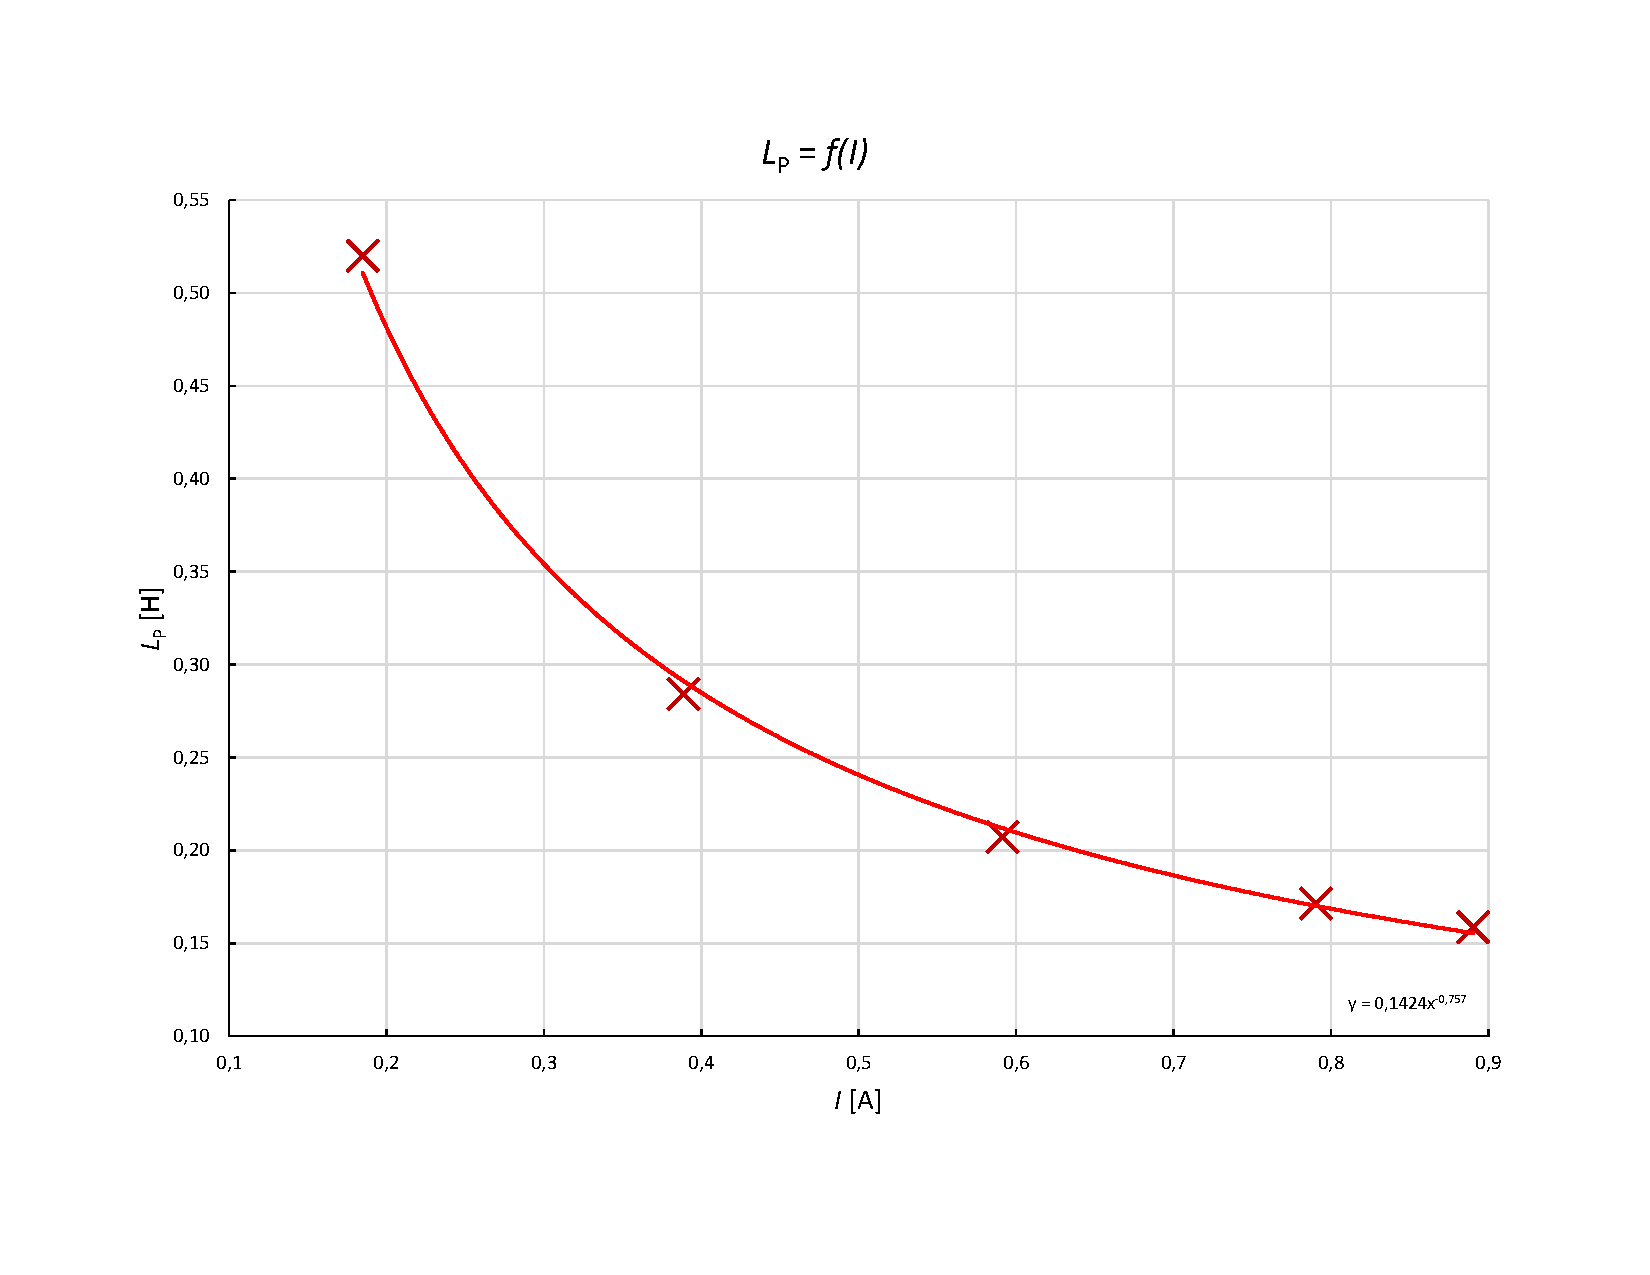
\includegraphics[width=\textwidth, trim={0 3cm 0 3cm}]{grafy/9A_graf2.pdf}
    \caption{Závislost hodnot $L_\text{P}$ paralelního náhradního schématu na sycení tlumivky}
\end{figure}

\begin{figure}[H]
    \centering
    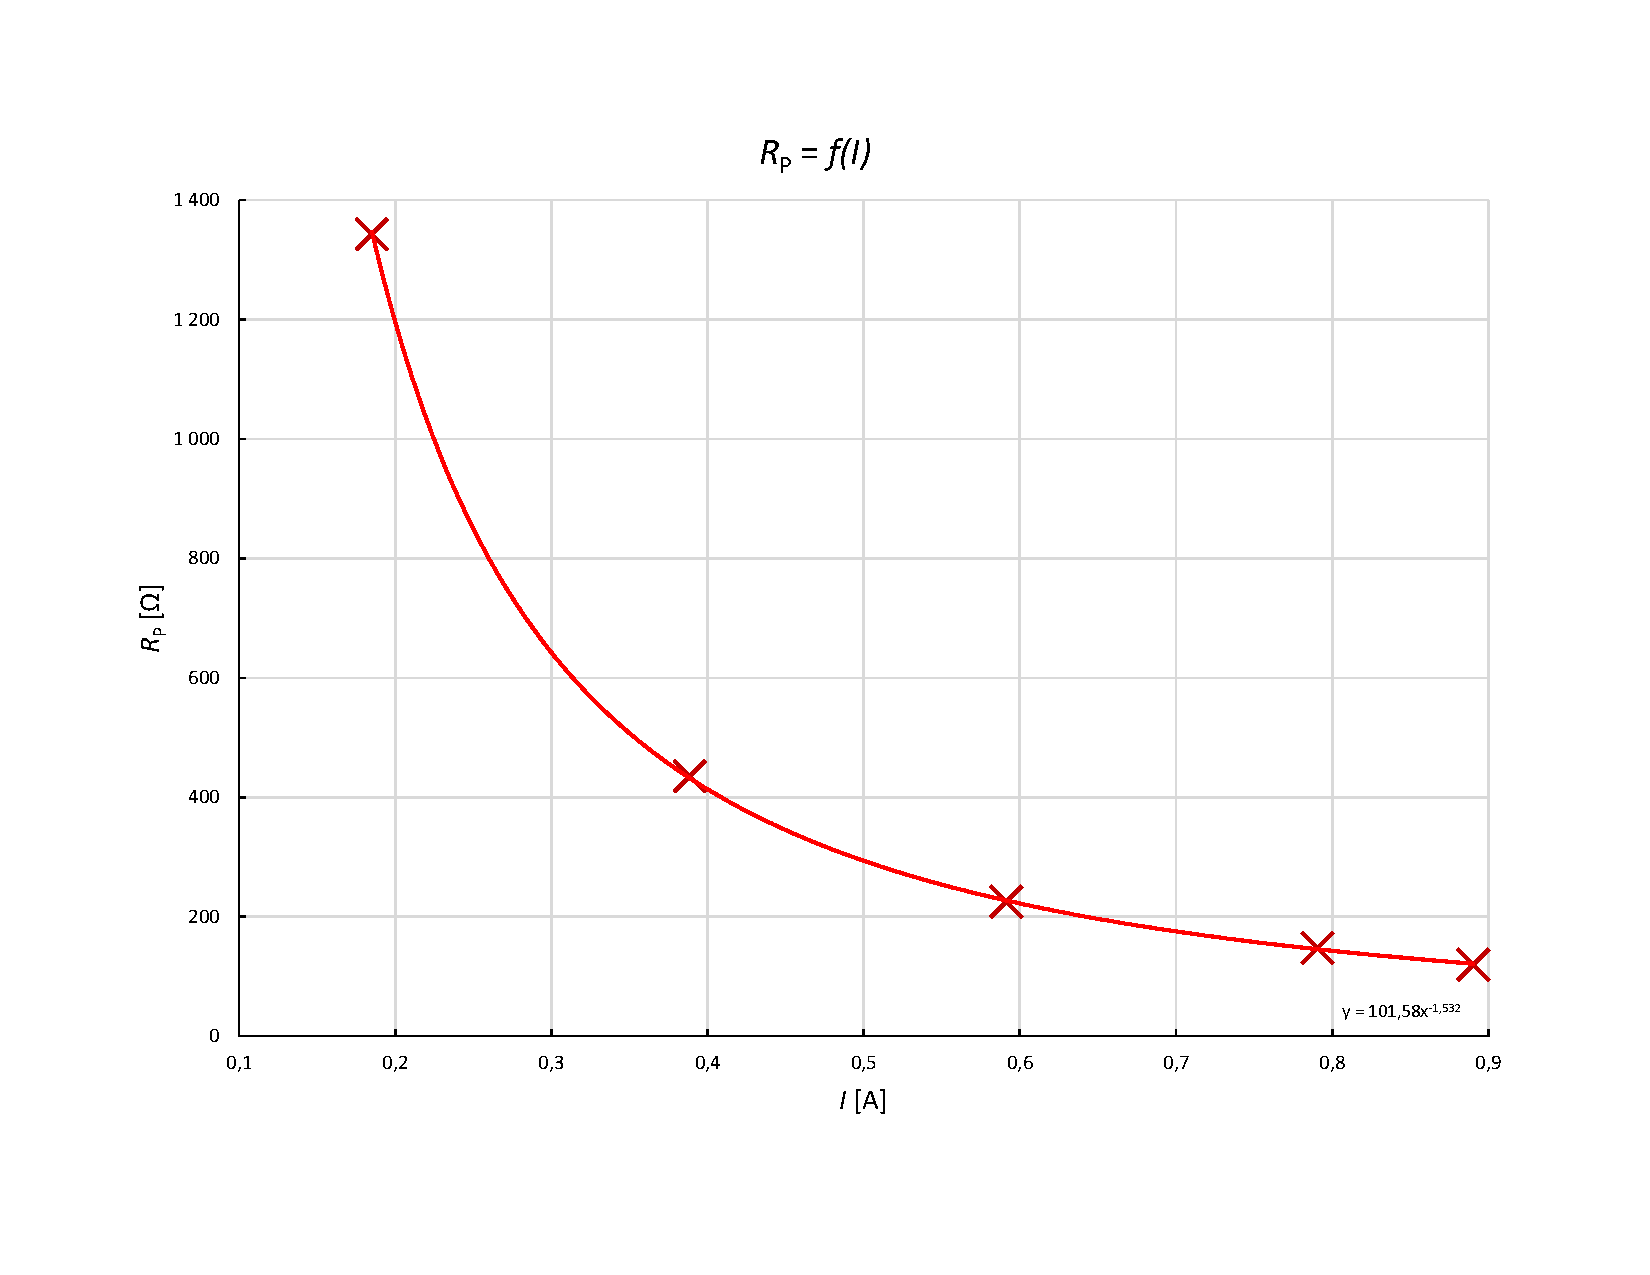
\includegraphics[width=\textwidth, trim={0 3cm 0 3cm}]{grafy/9A_graf1.pdf}
    \caption{Závislost hodnot $R_\text{P}$ paralelního náhradního schématu na sycení tlumivky}
\end{figure}

\subsection{Příklady výpočtu}

\begin{enumerate}
    \item Absolutní odchylka metody měření činného výkonu
    \begin{multline*}
        \Delta_P = \textcolor{teal}{U^2 \cdot \frac{R_\text{V} + R_\text{WU}}{R_\text{V} \cdot R_\text{WU}}}
        = \left(41\,V \right)^2 \cdot \frac{6\,000\,\Omega + 15\,000\,\Omega}{6\,000\,\Omega \cdot 15\,000\,\Omega} =
        \underline{\underline{0,392\,\text{W}}} \hfill
    \end{multline*}
    \item Korekce naměřeného činného výkonu
    \begin{multline*}
        P = \textcolor{teal}{P' - \Delta_P} = 14,4\,\text{W} - 0,392\,\text{W} = \underline{\underline{14,01\,\text{W}}} \hfill
    \end{multline*}
    \item Absolutní odchylka metody měření proudu
    \begin{multline*}
        \Delta_I = \textcolor{teal}{U \cdot \frac{R_\text{V} + R_\text{WU}}{R_\text{V} \cdot R_\text{WU}}}
        = 41\,V \cdot \frac{6\,000\,\Omega + 15\,000\,\Omega}{6\,000\,\Omega \cdot 15\,000\,\Omega} =
        \underline{\underline{0,010\,\text{A}}} \hfill
    \end{multline*}
    \item Korekce naměřeného proudu
    \begin{multline*}
        I = \textcolor{teal}{I_1 - \Delta_I} = 0,9\,\text{A} - 0,01\,\text{A} = \underline{\underline{0,89\,\text{A}}} \hfill
    \end{multline*}
    \item Parametry sériového náhradního obvodu
    \begin{multline*}
        R_\text{S} = \textcolor{teal}{\frac{P}{I^2}} = \frac{14,01\,\text{W}}{\left(0,89\,\text{A}\right)^2}
        = \underline{\underline{17,67\,\Omega}} \hfill \\
        \ \ \ L_\text{S} = \textcolor{teal}{\frac{1}{2 \pi f} \cdot \frac{\sqrt{U^2 \cdot I^2 - P^2}}{I^2}}
        = \frac{1}{2 \pi \cdot 50\,\text{Hz}} \cdot \frac{\sqrt{(41\,\text{V})^2 \cdot (0,89\,\text{A})^2 - (14,01\,\text{W})^2}}{(0,89\,\text{A})^2} = 
        \underline{\underline{0,135\,\text{H}}} \hfill
    \end{multline*}
    \item Parametry paralelního náhradního obvodu
    \begin{multline*}
        R_\text{S} = \textcolor{teal}{\frac{U^2}{P}} = \frac{(41\,\text{V})^2}{14,01\,\text{W}}
        = \underline{\underline{120\,\Omega}} \hfill \\
        \ \ \ L_\text{S} = \textcolor{teal}{\frac{1}{2 \pi f} \cdot \frac{U^2}{\sqrt{U^2 \cdot I^2 - P^2}}}
        = \frac{1}{2 \pi \cdot 50\,\text{Hz}} \cdot \frac{(41\,\text{V})^2}{\sqrt{(41\,\text{V})^2 \cdot (0,89\,\text{A})^2 - (14,01\,\text{W})^2}} = 
        \underline{\underline{0,159\,\text{H}}} \hfill
    \end{multline*}
    \item Nejistoty měření
    \begin{multline*}
        u_{BU} = \textcolor{teal}{\frac{\delta_{TP_V} \cdot X_R}{100 \% \cdot \chi}} = \frac{\delta_{TP_V} \cdot U_R}{100 \% \cdot \sqrt{3}} = \frac{0,5\% \cdot 60V}{100 \% \cdot \sqrt{3}} = \underline{\underline{0,1732\,\text{V}}} \hfill \\
        \ \ \ u_{BI} = \frac{\delta_{TP_A} \cdot I_R}{100 \% \cdot \sqrt{3}} = 346,4 \cdot 10^{-6} A = \underline{\underline{0,01732\,\text{A}}} \hfill \\
        \ \ \ u_{\text{B}P} = \textcolor{teal}{\sqrt{\left(p_\text{MTP}\,X_\text{RWU}\,X_\text{RWI}\,cos\,\varphi\,\frac{\delta_\text{TPW}}{100 \cdot \sqrt{3}}\right)^2 + \left(P \cdot \frac{\delta_\text{TP\,MTP}}{100 \cdot \sqrt{3}}\right)^2}} = \hfill \\
        \ \ \ = \sqrt{\left(0,2 \cdot 150 \cdot 5 \cdot 0,2 \cdot \frac{1}{100 \cdot \sqrt{3}}\right)^2 + \left(14,01 \cdot \frac{0,2}{100 \cdot \sqrt{3}}\right)^2} = \underline{\underline{0,1732\,\text{W}}} \hfill \\
        \ \ \ u_{R_\text{S}} = \textcolor{teal}{\sqrt{\left(\frac{1}{I^2} u_{\text{B}P}\right)^2 + \left(\frac{2P}{I^3}u_{\text{B}I}\right)^2}} = \sqrt{\left(\frac{1}{0,8916^2} 0,1732\right)^2 + \left(\frac{2 \cdot 14,01}{0,8916^3}0,01732\right)^2} = \underline{\underline{0,7764\,\Omega}} \hfill \\
        \ \ \ u_{L_S} = \textcolor{teal}{\cfrac{\sqrt{\left(\cfrac{P \cdot u_{BP}}{I^2}\right)^2 + \left(U \cdot u_{BU}\right)^2 + \left(\cfrac{\left(U^2I^2 - 2 P^2\right) \cdot u_{BI}}{I^3}\right)^2}}{2 \pi f \sqrt{U^2I^2-P^2}}} =  \hfill \\
        \ \ \ = \cfrac{\sqrt{\left(\cfrac{15,2472 \cdot 0,1732}{0,8916^2}\right)^2 + \left(41 \cdot 0,1732\right)^2 + \left(\cfrac{\left(41^2 \cdot 0,8916^2 - 2 \cdot 15,2472^2\right) \cdot 0,01732}{0,8916^3}\right)^2}}{2 \pi \cdot 50 \cdot \sqrt{41^2 \cdot 0,8916^2 - 15,2472^2}} = \underline{\underline{0,002258\,H}} \hfill \\
        \ \ \ u_{R_P} = \textcolor{teal}{\sqrt{\left(\frac{U^2}{P^2}u_{BP}\right)^2 + \left(\frac{2U}{P}u_{BU}\right)^2}} = \sqrt{\left(\frac{42^2}{15,2472^2}0,1732\right)^2 + \left(\frac{2 \cdot 42}{15,2472}0,1732\right)^2} = \underline{\underline{1,1641\,\Omega}} \hfill \\
        \ \ \ u_{L_P} = \textcolor{teal}{\cfrac{\sqrt{(U^2 \cdot P \cdot u_{BP})^2 + (U \cdot (U^2I^2 - 2P^2) \cdot u_{BU})^2 + (U^4\cdot I \cdot u_{BI})^2}}{2 \pi f \sqrt{U^2I^2-P^2}}} = \hfill \\
        \ \ \ = \cfrac{\sqrt{(42^2 \cdot 15,2472 \cdot 0,1732)^2 + (42 \cdot (42^2 \cdot 0,8916^2 - 2 \cdot 15,2472^2) \cdot 0,1732)^2 + (42^4\cdot 0,8916 \cdot 0,01732)^2}}{2 \pi 50 \cdot \sqrt{42^2 \cdot 0,8916^2-15,2472^2}} = \hfill \\
        \ \ \ = \underline{\underline{0,00879\,\text{H}}} \hfill \\
        \ \ \ \tilde{U}_{R_S} = \textcolor{teal}{\frac{k_r \cdot u_{R_S}}{R_S} \cdot 100\,\%} = \frac{2 \cdot 0,7764}{17,67} \cdot 100\,\% = \underline{\underline{8,1\,\%}} \hfill \\
        \ \ \ \tilde{U}_{L_S} = \textcolor{teal}{\frac{k_r \cdot u_{L_S}}{L_S} \cdot 100\,\%} = \frac{2 \cdot 0,00258}{0,135} \cdot 100\,\% = \underline{\underline{3,3\,\%}} \hfill \\
        \ \ \ \tilde{U}_{R_P} = \textcolor{teal}{\frac{k_r \cdot u_{R_P}}{R_P} \cdot 100\,\%} = \frac{2 \cdot 1,624}{120} \cdot 100\,\% = \underline{\underline{2,81\,\%}} \hfill \\
        \ \ \ \tilde{U}_{L_P} = \textcolor{teal}{\frac{k_r \cdot u_{L_P}}{L_P} \cdot 100\,\%} = \frac{2 \cdot 0,003879}{0,159} \cdot 100\,\% = \underline{\underline{4,73\,\%}} \hfill
    \end{multline*}
\end{enumerate}

\section{Seznam použitých přístrojů}

\section{Závěr}

\end{document}